\documentclass{beamer}
\usetheme{metropolis}
\usepackage{tikz}
\usepackage{booktabs}

\title{A Beamer presentation}
\author{ofree-engine}

\begin{document}
\begin{frame}
  \titlepage
\end{frame}

\begin{frame}{Outline}
  \tableofcontents
\end{frame}

\section{Results}
\begin{frame}{Overlays}
  \begin{itemize}
    \item<1-> First point
    \item<2-> Second point
  \end{itemize}
  \pause
  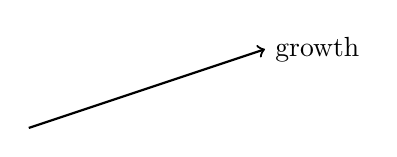
\begin{tikzpicture}
    \draw[->, thick] (0,0) -- (3,1) node[right] {growth};
  \end{tikzpicture}
\end{frame}

\begin{frame}{A table}
  \centering
  \begin{tabular}{lr}
    \toprule Method & Score \\ \midrule A & 0.91 \\ B & 0.87 \\ \bottomrule
  \end{tabular}
\end{frame}
\end{document}
